%
% ---- Technologies
%

\section{Technologies}\label{sec:technologies}

%
% ---- Choice of technologies in scope
%
\subsection{Scope}
\subsubsection{In Scope.}  The selected technologies in scope of this paper are shared middleware queues, distributed databases and microservices, which are discussed in more detail below.  The database partitioning strategy and entirely separate databases for the microservices architecture offer alternative means of isolating the skewed demand.  Using a single middleware queue shares and distributes the demand, this time in contrast to the microservices middleware approach.  The models will compare these approaches and investigate the behaviour of systems where the components have conflicting approaches to handling demand.
\subsubsection{Out of Scope.}  The paper will not consider elastic scaling or HTTP load balancing.  There is already a great deal of work in evaluating right-sizing strategies (minimising underutilisation and overutilisation of compute resources) for the former, e.g. \cite{RN49}, \cite{RN62}, \cite{RN48}.  HTTP load balancing is a relatively mature technology, and work has been done on simulation to evaluate different algorithms by response time and web server utilisation \cite{RN55}.

%
% ---- Queue Middleware
%

\subsection{Queue Middleware}\label{sec:middleware}

Good choice of middleware in a system will help ensure that its components are connected, but loosely coupled.  If, for example, a web server is blocked waiting for a response from a worker application carrying out a more expensive operation, then the throughput of the web server will be limited to that of the worker application.  The use case `return' operation however does not require a direct response from the system.  As long as the customer can rely on eventual guaranteed delivery of the return request, (and that the cost of their ticket will be refunded) then they do not need to wait for a direct response to their return.

Point-to-Point Queues, e.g. Azure Storage Queues \cite{RN1072}, are a form of Message-Oriented Middleware - an asynchronous, brokered message service providing an intermediate layer between senders and receivers, decoupling their communication.  Message delivery may take minutes rather than milliseconds, but the service providers do provide configurable delivery guarantees \cite{RN65}.  With synchronous middleware such as Remote Procedure Call (RPC), the calling process is blocked until the called service completes and returns control to the caller.  Distributed systems using asynchronous middleware do not block when calling a remote service.  Control is immediately passed back to the caller, and a response may be returned eventually, with the caller polling the remote service for the response, or the remote process calling a method in the caller to send the response.

Many processes may send messages to a queue, and each message is received by one consumer - though it may be one of several consumers competing for messages from this queue.  This competing consumer pattern offers a means of balancing load from the Web Servers between the Worker Applications in the ticketing use case.

%
% ---- Microservices
%
\FloatBarrier
\subsection{Microservices}\label{sec:microservices}

Microservices architecture is an approach to structuring applications as suites of small services, defined by business capability verticals rather than technological layers \cite{RN1069} \cite{RN1070}.  Each of the use case requirements - search for, book or return tickets - might typically be microservices with their own worker applications and data nodes.  Ticket data would be denormalised across the data nodes and made eventually consistent via a backplane messaging service \cite{RN1071} as shown in Figure \ref{figure:microservices}.  This would certainly isolate the demand for search, book and return from each other - returning tickets would not be blocked by a system where bookings were overloaded.  In the ticketing use case however, there is skewed demand for athletics tickets.  In a real-world system the booking microservice might be further broken down to a lower level of granularity to deal with this, i.e. a separate microservice for booking each ticket type.

\begin{figure}
	\label{figure:microservices}
	\centering
	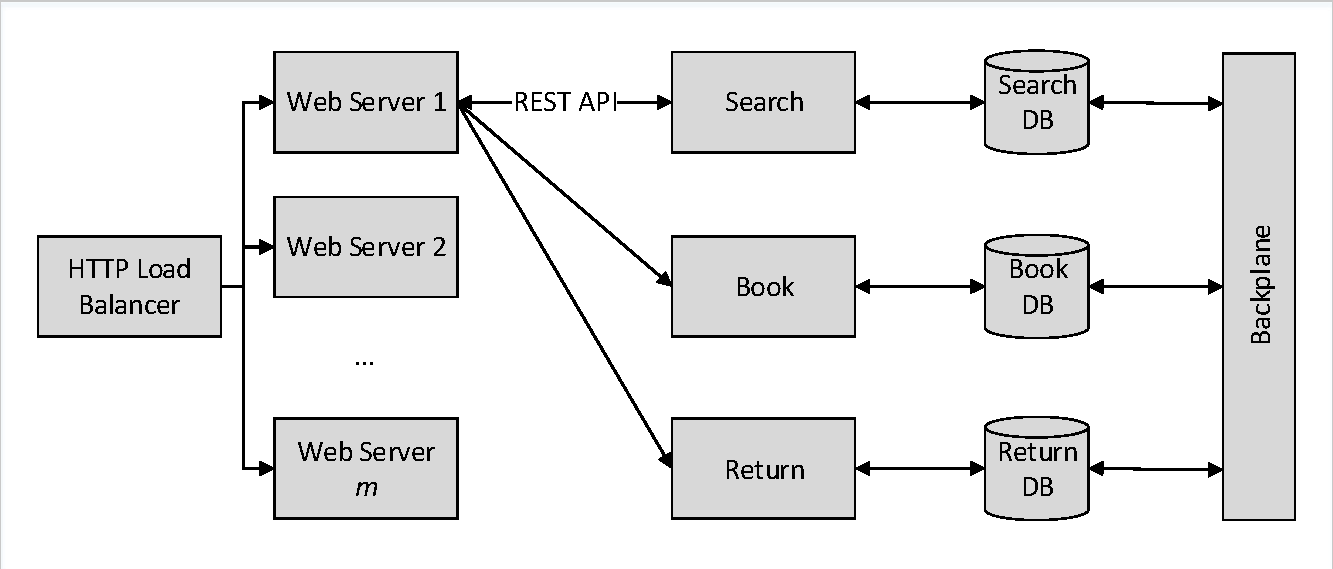
\includegraphics[trim = 5 5 5 5, clip, width=\textwidth]{img/microservices}
	\caption{Microservices}
\end{figure}

%
% ---- Distributed databases
%
\FloatBarrier
\subsection{Distributed databases}\label{sec:distributed-databases}
Modern SQL and NoSQL databases are designed to scale both data and the load of operations accessing that data over many servers that do not share disk or RAM, so-called `shared nothing' architecture \cite{RN67}.  We may partition data {\itshape vertically}, dividing tables into groups of columns that may be placed on different data nodes; or {\itshape horizontally}, where the split is by row \cite{RN68}. 

In the use case, the quantity of data does not approach the levels of `Big Data' applications.  Partitioning is proposed instead as a means of scaling the demand for that data.  The ticketing system will not require a large number of columns and the three operations outlined do not have significantly different column requirements, therefore horizontal partitioning is most relevant.  The partition key of a Ticket table may be the Ticket Type, the Date, or the seat Row.  Demand for tickets is likely to vary by each of these attributes.  An alternative partitioning strategy would be to on denormalised tables supporting the query, book and return operations.  The load on each data node would follow the demand for the data types and operations placed there.

One issue to be aware of is {\itshape replication}.   Most distributed databases offer replication of data from one partition to another for availability.  In the use case, if demand overloads a data node, the database may share the throughput using a copy of the data on another data node.  If this is also the primary data node of an otherwise low demand data type, then it may be overwhelmed in turn i.e. the skewed demand has followed the data.

\begin{figure}
	\label{figure:consistent_hashing}
	\centering
	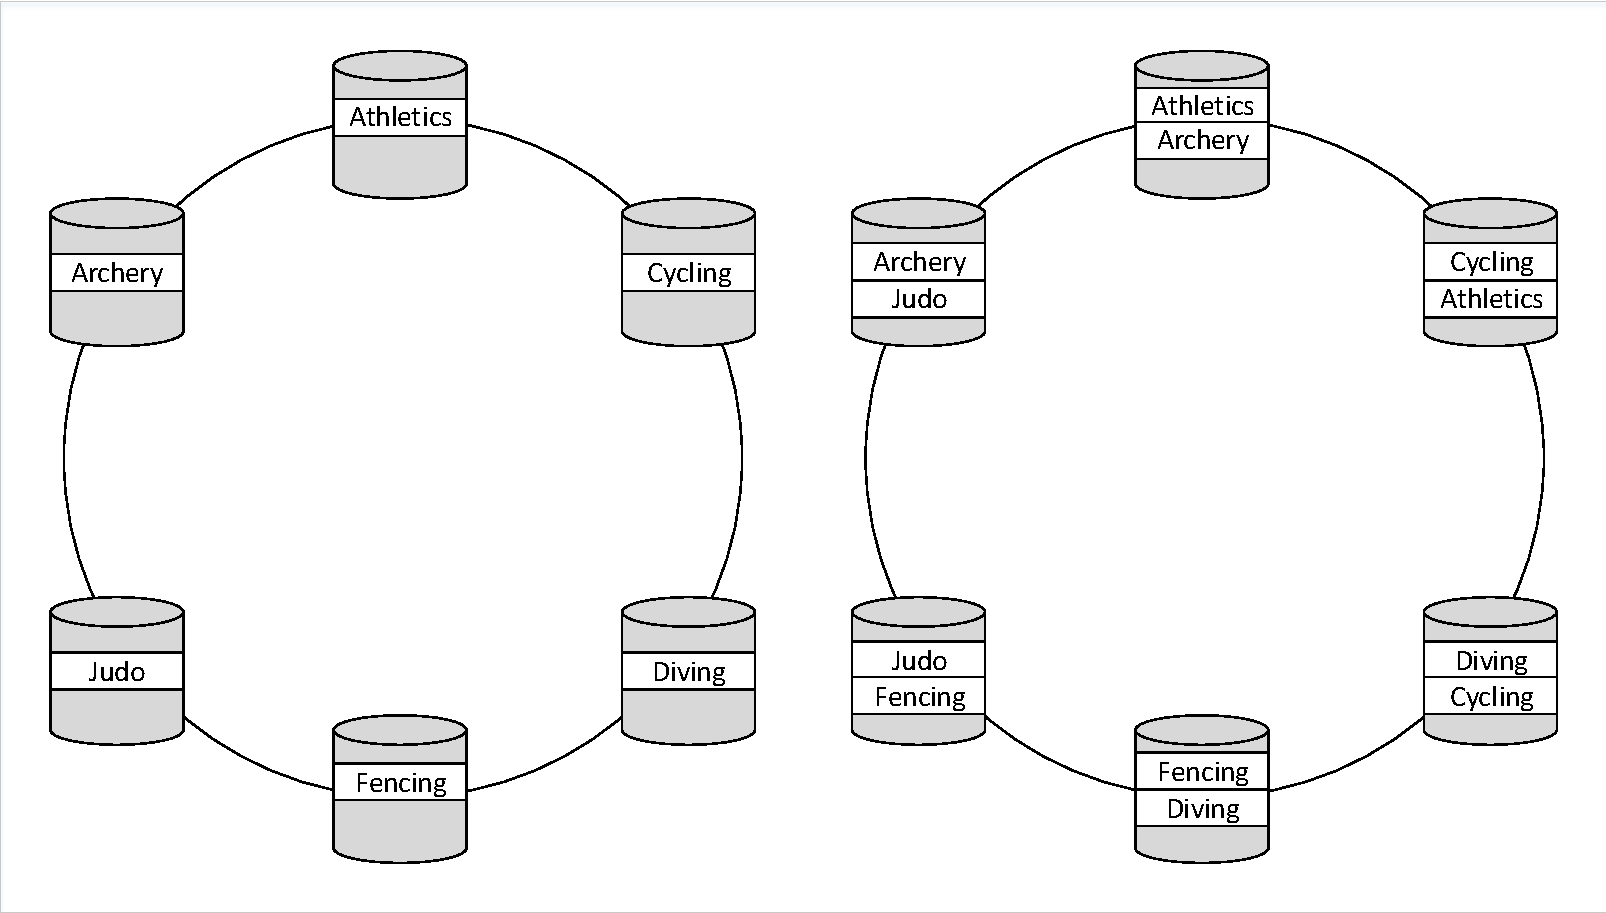
\includegraphics[trim = 5 5 5 5, clip, width=\textwidth]{img/dbdist}
	\caption{Consistent hashing, without and with replication}
\end{figure}
\FloatBarrier
The Cassandra database has an interesting method of partitioning data, using {\itshape consistent hashing} (also used by Riak, Redis and BigData among others \cite{RN66}).  The largest output of a hash function wraps round to the smallest value so that the range of hash values forms a conceptual `ring'.  Each data node is assigned a position on this ring, then the hash value of the partition key of a data item is used to determine the node used to store it.  When using replication, with a replication factor of {\itshape N}, a copy of the data is placed on the next {\itshape N-1} nodes walking clockwise round the ring \cite{RN1050}.  This is illustrated in Figure \ref{figure:consistent_hashing}.
